\documentclass[%
  10pt,% default; alternatives: 11pt, 12pt, 14pt
  %handout,% flatten overlays for the sake of printed handouts
]{../templates/pres_template/cognigronbeamer}


\usepackage{graphicx}
\usepackage{ragged2e}
\usepackage{textcomp} % ensures TS1 symbols are available
\DeclareTextSymbolDefault{\textbullet}{TS1}

% for the frame header:
\facname{Faculty of Science\\ and Engineering} % optional
\group{Bio-inspired\\ Circuits and Systems} % optional
\inst{cognigron} % optional
\date{\today}
% \extralogo{...} % disabled in image-free version

% for the title frame:
\title{A Title}
\subtitle{RUG beamer-based presentations}
\author{A. Uthor}
\institute{University of Groningen\\ Faculty of Science and Engineering}

\begin{document}

% title slide
{
\setbeamertemplate{background canvas}{\titleback}
\begin{frame}%[plain]
\titlepage
\end{frame}
}


\section{13/04/2026}


\begin{frame}
  set up this repository for all of my thesis work. going to attempt to set up obsidian maybe as well.
  % clone with "git clone https://github.com/EricJSHallen/sebastian_thesis_repo/tree/master"
\end{frame}

\begin{frame}
  Translinear Principle
  \begin{itemize}
    \item \(\sum_{n\epsilon CW}V_n = \sum_{n\epsilon CCW}V_n\)
    \item \(\prod_{n \in \mathrm{CW}} I_n = \prod_{n \in \mathrm{CCW}} I_n\)
    \item Valid for BJT's and MOSFET under weak inversion regime.
  \end{itemize}
  \begin{figure}
    % \raggedright
    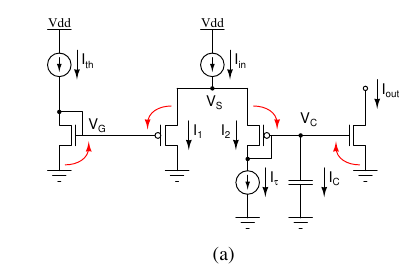
\includegraphics[width=0.35\textwidth]{DPI1eg.png}
  \end{figure}
\end{frame}

\begin{frame}
  inversion regime's
  \begin{itemize}
    \item weak inversion: sparse inversion layer???, diffusion transport
    \item moderate inversion: 
    \item strong inversion: well formed channel????, drift transport
  \end{itemize}
\end{frame}


\begin{frame}
  Log domain cirtucits
  \begin{itemize}
    \item circuits that can be described by linear differential equations despite having nonlinear internal components
    \item why are they called "Log domain"???
  \end{itemize}
\end{frame}



\begin{frame}
  Technical questions
  \begin{itemize}
    \item Latex(VScode) how to interupt compiling operation if system is hung (stuck on wpmain.synctex(busy)) typically?
  \end{itemize}
  Admin questions
  \begin{itemize}
    \item should I upload pdf's of all of my scanned notes that I have taken thusfar to this repository so that it is available?
    \item could I send you a copy of the presentation I make for the group meeting thursday before I present?
  \end{itemize}
  random theory questions
  \begin{itemize}
    \item If I understand this correctly when you refer to "maintaining the linear dynamics" as we go from n dynapses to 1 dynapse, that is the system is still "log domain" assuming I understood that principal correctly?
  \end{itemize}
\end{frame}

\begin{frame}
  Goals for friday 17th (and Thursday 16th)
  \begin{itemize}
    \item prepare presentation for the thursday meeting
    \item read chapter 5 VLSI and take notes on it
    \item read "Lab V - DPI Synapse and Axon-Hillock Neuron" write down list of questions.
    \item schedule meeting with masters student in Zurich (send message after this meeting)
    \item get in contact with the other BSc student? 
    \item priority reading list?? get through the 3 most important papers (if possible more)
    \item recreate the circuits provided to me 
  \end{itemize}
\end{frame}

% % section slide
% \section{Big Menu}
% %\label{sec:samples}

% % standard slide
% \begin{frame}
%   \frametitle{Today's menu}
%   Today we have a special menu.
% \end{frame}

% % itemize slide
% \begin{frame}{Today's menu - first course}
%   \begin{itemize}
%     \item soup
%       \begin{itemize}
%       \item tortilla filled with meat and vegetables
%       \item refried beans
%       \end{itemize}
%   \end{itemize}
% \end{frame}

% % Stepped enumerated list with pause
% \begin{frame}{Stepped enumerated list with {\ttfamily pause}}
%   \begin{enumerate}
%     \item Is the soup good?\pause
%     \item Is the main course good?\pause
%     \item Are the tortillas good?
%   \end{enumerate}
% \end{frame}



% % empty background; put inside braces to localize background redefinition
% {
% \setbeamertemplate{background canvas}{}
% \begin{frame}[plain]{Empty background example}
%   Empty background
% \end{frame}
% }



\end{document}